% Options for packages loaded elsewhere
\PassOptionsToPackage{unicode}{hyperref}
\PassOptionsToPackage{hyphens}{url}
\PassOptionsToPackage{dvipsnames,svgnames,x11names}{xcolor}
%
\documentclass[
  8pt,
  12pt]{article}

\usepackage{amsmath,amssymb}
\usepackage{iftex}
\ifPDFTeX
  \usepackage[T1]{fontenc}
  \usepackage[utf8]{inputenc}
  \usepackage{textcomp} % provide euro and other symbols
\else % if luatex or xetex
  \usepackage{unicode-math}
  \defaultfontfeatures{Scale=MatchLowercase}
  \defaultfontfeatures[\rmfamily]{Ligatures=TeX,Scale=1}
\fi
\usepackage{lmodern}
\ifPDFTeX\else  
    % xetex/luatex font selection
\fi
% Use upquote if available, for straight quotes in verbatim environments
\IfFileExists{upquote.sty}{\usepackage{upquote}}{}
\IfFileExists{microtype.sty}{% use microtype if available
  \usepackage[]{microtype}
  \UseMicrotypeSet[protrusion]{basicmath} % disable protrusion for tt fonts
}{}
\makeatletter
\@ifundefined{KOMAClassName}{% if non-KOMA class
  \IfFileExists{parskip.sty}{%
    \usepackage{parskip}
  }{% else
    \setlength{\parindent}{0pt}
    \setlength{\parskip}{6pt plus 2pt minus 1pt}}
}{% if KOMA class
  \KOMAoptions{parskip=half}}
\makeatother
\usepackage{xcolor}
\setlength{\emergencystretch}{3em} % prevent overfull lines
\setcounter{secnumdepth}{5}
% Make \paragraph and \subparagraph free-standing
\makeatletter
\ifx\paragraph\undefined\else
  \let\oldparagraph\paragraph
  \renewcommand{\paragraph}{
    \@ifstar
      \xxxParagraphStar
      \xxxParagraphNoStar
  }
  \newcommand{\xxxParagraphStar}[1]{\oldparagraph*{#1}\mbox{}}
  \newcommand{\xxxParagraphNoStar}[1]{\oldparagraph{#1}\mbox{}}
\fi
\ifx\subparagraph\undefined\else
  \let\oldsubparagraph\subparagraph
  \renewcommand{\subparagraph}{
    \@ifstar
      \xxxSubParagraphStar
      \xxxSubParagraphNoStar
  }
  \newcommand{\xxxSubParagraphStar}[1]{\oldsubparagraph*{#1}\mbox{}}
  \newcommand{\xxxSubParagraphNoStar}[1]{\oldsubparagraph{#1}\mbox{}}
\fi
\makeatother


\providecommand{\tightlist}{%
  \setlength{\itemsep}{0pt}\setlength{\parskip}{0pt}}\usepackage{longtable,booktabs,array}
\usepackage{calc} % for calculating minipage widths
% Correct order of tables after \paragraph or \subparagraph
\usepackage{etoolbox}
\makeatletter
\patchcmd\longtable{\par}{\if@noskipsec\mbox{}\fi\par}{}{}
\makeatother
% Allow footnotes in longtable head/foot
\IfFileExists{footnotehyper.sty}{\usepackage{footnotehyper}}{\usepackage{footnote}}
\makesavenoteenv{longtable}
\usepackage{graphicx}
\makeatletter
\def\maxwidth{\ifdim\Gin@nat@width>\linewidth\linewidth\else\Gin@nat@width\fi}
\def\maxheight{\ifdim\Gin@nat@height>\textheight\textheight\else\Gin@nat@height\fi}
\makeatother
% Scale images if necessary, so that they will not overflow the page
% margins by default, and it is still possible to overwrite the defaults
% using explicit options in \includegraphics[width, height, ...]{}
\setkeys{Gin}{width=\maxwidth,height=\maxheight,keepaspectratio}
% Set default figure placement to htbp
\makeatletter
\def\fps@figure{htbp}
\makeatother

\addtolength{\oddsidemargin}{-.5in}%
\addtolength{\evensidemargin}{-1in}%
\addtolength{\textwidth}{1in}%
\addtolength{\textheight}{1.7in}%
\addtolength{\topmargin}{-1in}%
\makeatletter
\@ifpackageloaded{caption}{}{\usepackage{caption}}
\AtBeginDocument{%
\ifdefined\contentsname
  \renewcommand*\contentsname{Table of contents}
\else
  \newcommand\contentsname{Table of contents}
\fi
\ifdefined\listfigurename
  \renewcommand*\listfigurename{List of Figures}
\else
  \newcommand\listfigurename{List of Figures}
\fi
\ifdefined\listtablename
  \renewcommand*\listtablename{List of Tables}
\else
  \newcommand\listtablename{List of Tables}
\fi
\ifdefined\figurename
  \renewcommand*\figurename{Figure}
\else
  \newcommand\figurename{Figure}
\fi
\ifdefined\tablename
  \renewcommand*\tablename{Table}
\else
  \newcommand\tablename{Table}
\fi
}
\@ifpackageloaded{float}{}{\usepackage{float}}
\floatstyle{ruled}
\@ifundefined{c@chapter}{\newfloat{codelisting}{h}{lop}}{\newfloat{codelisting}{h}{lop}[chapter]}
\floatname{codelisting}{Listing}
\newcommand*\listoflistings{\listof{codelisting}{List of Listings}}
\makeatother
\makeatletter
\makeatother
\makeatletter
\@ifpackageloaded{caption}{}{\usepackage{caption}}
\@ifpackageloaded{subcaption}{}{\usepackage{subcaption}}
\makeatother
\ifLuaTeX
  \usepackage{selnolig}  % disable illegal ligatures
\fi
\usepackage[]{natbib}
\bibliographystyle{agsm}
\usepackage{bookmark}

\IfFileExists{xurl.sty}{\usepackage{xurl}}{} % add URL line breaks if available
\urlstyle{same} % disable monospaced font for URLs
\hypersetup{
  pdftitle={Zoning: A Barrier or Solution to Truck Parking Infrastructure Shortages?},
  pdfauthor={William Co},
  colorlinks=true,
  linkcolor={blue},
  filecolor={Maroon},
  citecolor={Blue},
  urlcolor={Blue},
  pdfcreator={LaTeX via pandoc}}


\begin{document}


\def\spacingset#1{\renewcommand{\baselinestretch}%
{#1}\small\normalsize} \spacingset{1}


%%%%%%%%%%%%%%%%%%%%%%%%%%%%%%%%%%%%%%%%%%%%%%%%%%%%%%%%%%%%%%%%%%%%%%%%%%%%%%

\date{March 10, 2025}
\title{\bf Zoning: A Barrier or Solution to Truck Parking Infrastructure
Shortages?}
\author{
William Co\thanks{true}\\
Department of Economics, University of British Columbia\\
}
\maketitle

\bigskip
\bigskip
\begin{abstract}

\end{abstract}


\newpage
\spacingset{1.9} % DON'T change the spacing!

\section{Results and Interpretations}\label{results-and-interpretations}

\begin{figure}

\centering{

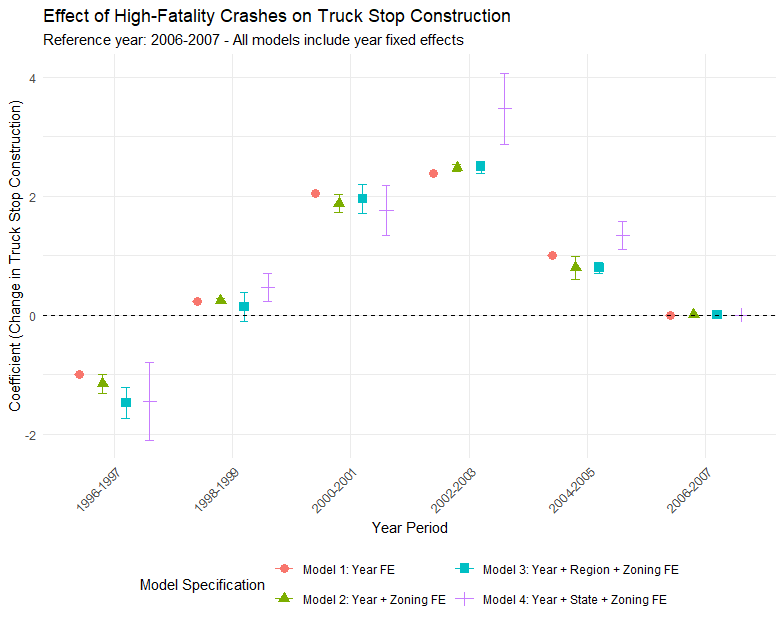
\includegraphics[width=5.67708in,height=\textheight]{images/Rplot.png}

}

\caption{\label{fig-time}Time Coefficients of Event Study Model}

\end{figure}%

\begin{figure}

\centering{

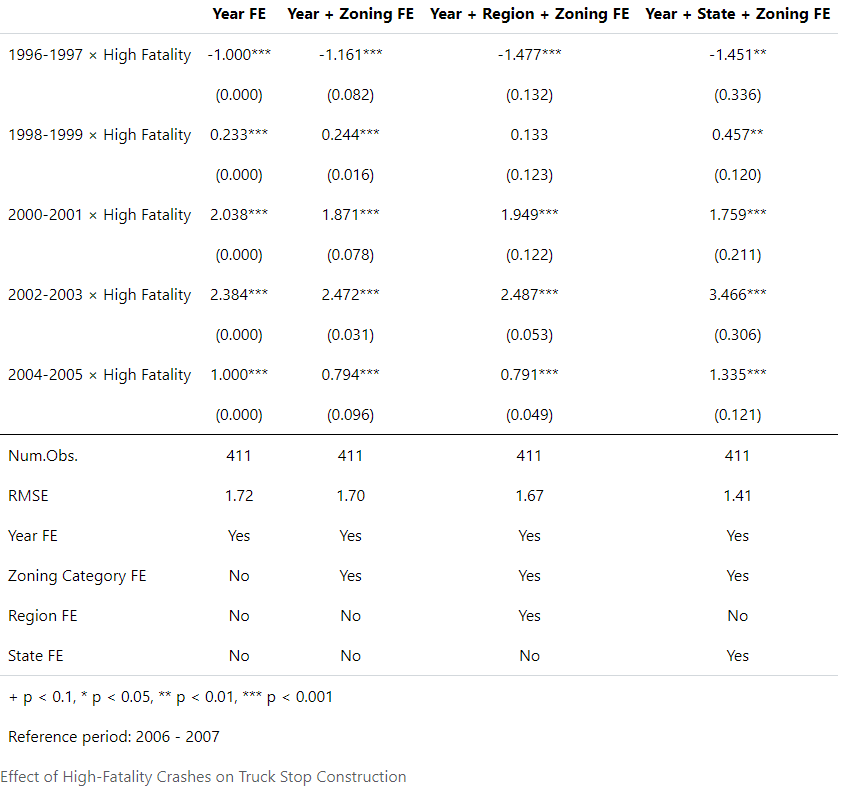
\includegraphics[width=5.59375in,height=\textheight]{images/Screenshot 2025-03-09 225540.png}

}

\caption{\label{fig-SummaryTable}Summary Table of Time Coefficients}

\end{figure}%

\subsection{Time Coefficients of Event Study
Model}\label{time-coefficients-of-event-study-model}

Figure~\ref{fig-SummaryTable} presents the estimated coefficients from
an event study model analyzing the relationship between high-fatality
truck crashes and subsequent truck stop construction across four
specifications. All models include year fixed effects, with progressive
controls for zoning, region, and state fixed effects. The reference
period is 2006--2007.

The interaction terms for high-fatality crashes exhibit statistically
significant positive coefficients across most time periods, robustly
rejecting the null hypothesis of no policy response to accidents. The
most pronounced effects occur in the 2002--2003 × High Fatality
interaction, with coefficients ranging from 2.384*** (Model 1, baseline)
to 3.466*** (Model 4, state and zoning FE). These magnitudes imply that
localities exposed to high-fatality crashes in 2002--2003 constructed
approximately 2.4 to 3.5 additional truck stops over the subsequent
decade, relative to the reference period. The lagged response aligns
with infrastructure development timelines, as the 2002--2003 effects
likely reflect construction initiated in response to crashes occurring 5
years prior, consistent with planning, permitting, and construction
phases.

Coefficients for 2000--2005 interactions are uniformly positive and
statistically significant (p \textless{} 0.001 in most specifications).
For instance, Model 3 (year, region, and zoning FE) yields a coefficient
of 2.487*** for 2002--2003, suggesting localities increased truck stop
supply by roughly 2.5 units over ten years following a high-fatality
crash. The results are robust across specifications, with declining RMSE
(1.72 to 1.41) and stable significance levels as fixed effects are
added.

\begin{figure}

\centering{

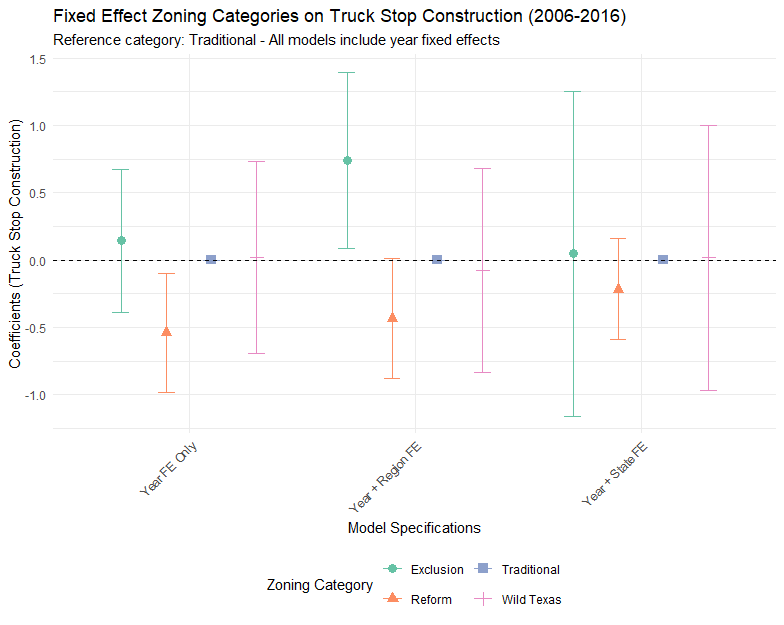
\includegraphics[width=6.01042in,height=\textheight]{images/Rplot01.png}

}

\caption{\label{fig-zonign_categories}Zoning Category Coefficients Plot}

\end{figure}%

\begin{figure}

\centering{

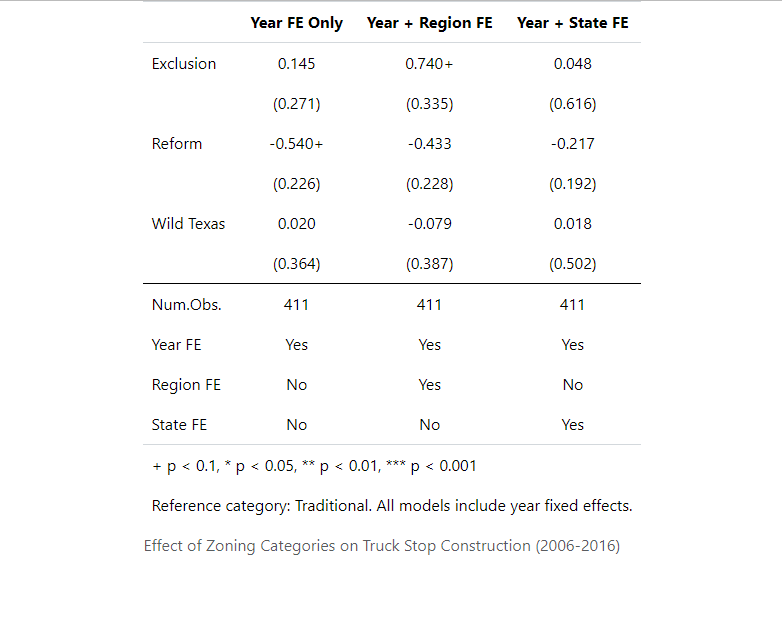
\includegraphics[width=5.78125in,height=\textheight]{images/Rplot05.png}

}

\caption{\label{fig-zoning_table}Zoning Category Coefficients Table}

\end{figure}%

\subsection{Zoning Category and Fixed
Effects}\label{zoning-category-and-fixed-effects}

Figure~\ref{fig-zoning_table} and Figure~\ref{fig-zonign_categories}
present coefficient estimates for zoning categories across three model
specifications, revealing findings that challenge initial hypotheses.
Contrary to expectations, zoning category fixed effects exhibit
negligible explanatory power, with coefficients for Exclusion, Reform,
and Wild Texas zones remaining statistically insignificant in nearly all
models. This undermines assumptions that restrictive zoning (e.g.,
Exclusion zones) systematically constrains construction or that
liberalized zoning (Reform zones) consistently facilitates it. For
Exclusion Zones, coefficients are insignificant in Model 1 (0.145,
p=0.271) and Model 3 (0.048, p=0.616), with only a marginally positive
effect in Model 2 (0.740+, p\textless0.1), suggesting limited evidence
of regulatory suppression. Similarly, Reform Zones show a marginally
negative coefficient in Model 1 (-0.540+, p\textless0.1), but this
effect disappears when region or state-level fixed effects are
introduced, implying that spatial heterogeneity rather than zoning
itself may drive observed patterns. Wild Texas Zones further reinforce
null results, with coefficients consistently near zero (e.g., -0.079 in
Model 2, p=0.387). Collectively, these results question the presumed
causal role of zoning categories in shaping construction outcomes,
highlighting the need to consider alternative mechanisms.

\begin{figure}

\centering{

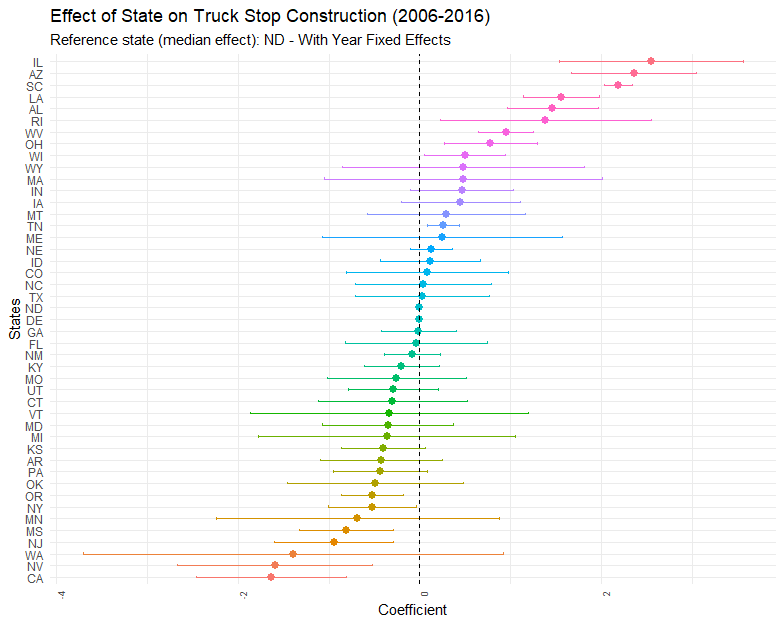
\includegraphics[width=6.19792in,height=\textheight]{images/Rplot04.png}

}

\caption{\label{fig-StateZoning}Coefficient of State Fix Effect}

\end{figure}%

Figure~\ref{fig-StateZoning} presents the estimated state fixed effects
on truck stop construction between 2006 and 2016, with North Dakota
serving as the reference category. The coefficients represent deviations
from the median effect, accounting for year fixed effects.

Economically, states with significantly positive coefficients, such as
Illinois and Arizona, may have more favorable regulatory environments,
higher demand for truck stops, or less restrictive zoning laws.
Conversely, states with large negative coefficients, such as California
and New York, likely impose stricter land-use regulations, face higher
land costs, or have geographical constraints limiting truck stop
expansion.

The confidence intervals indicate the statistical uncertainty around
these estimates. Wider intervals suggest greater variability in truck
stop construction within a state, potentially due to heterogeneous local
policies or smaller sample sizes.

\begin{figure}

\centering{

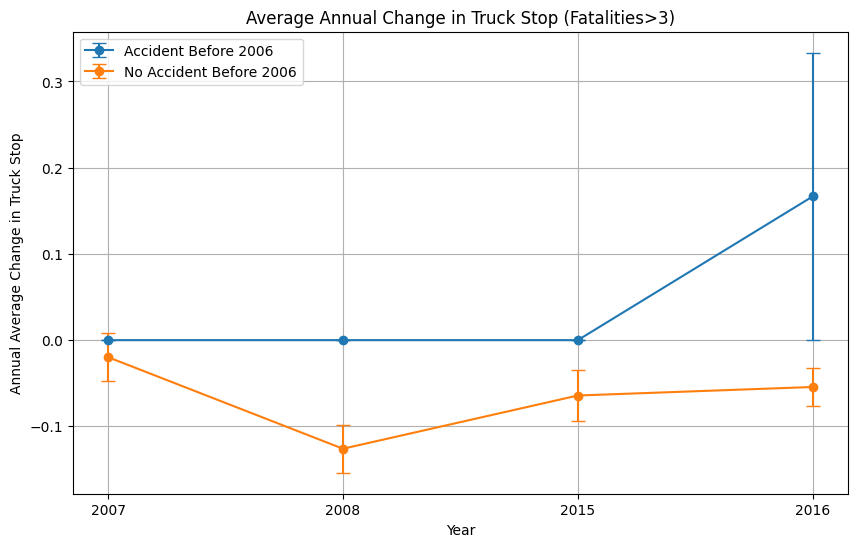
\includegraphics[width=4.6875in,height=\textheight]{images/output.png}

}

\caption{\label{fig-trends_past}Parallel Trends Counties with accident
Against without accident before 2006}

\end{figure}%

\begin{figure}

\centering{

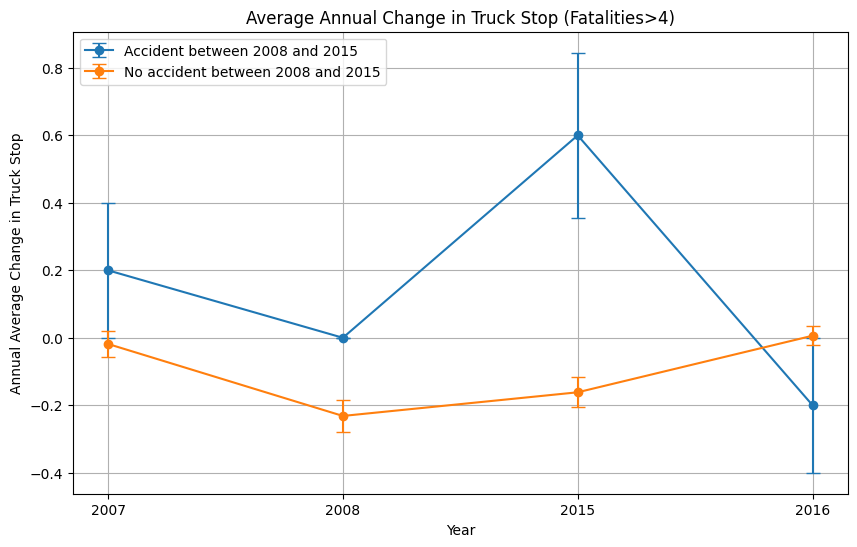
\includegraphics[width=4.71875in,height=\textheight]{images/output-01.png}

}

\caption{\label{fig-trends_mid}Parallel Trends Counties with accident
Against without accident between 2008 and 2015}

\end{figure}%

\subsection{Parallel Trends}\label{parallel-trends}

The results suggest that pre-treatment trends in truck stop construction
are similar across treated and control group. In
Figure~\ref{fig-trends_past}, counties that experienced high-fatality
accidents before 2006 consistently exhibit a higher rate of truck stop
construction relative to counties without such accidents. This is
expected, given that accidents could signal a need for increased
infrastructure, reinforcing our estimates. Meanwhile,
Figure~\ref{fig-trends_mid} demonstrates parallel trends before the
accident period (2008-2015). After 2015, a clear divergence emerges,
with accident-prone counties experiencing a sharp increase in truck stop
construction (+0.6 annual change). This pattern supports a causal
interpretation: post-accident infrastructure responses drive the
observed increase, rather than pre-existing trends or omitted variables.
These results suggest that bias due to non-parallel pre-treatment trends
is unlikely to be a significant issue.

\subsection{Bias}\label{bias}

A potential source of \emph{downward bias} in our estimates arises from
unobserved capacity expansions at existing truck stops. Because the data
set captures only new construction (i.e., the establishment of
additional truck stops) rather than expansions of current facilities,
any increase in capacity that does not involve constructing an entirely
new site remains unaccounted for. As a result, the observed impact on
truck stop supply may be understated relative to the true effect.

Additionally, concerns might arise regarding the time variation of
zoning classifications. However, empirical evidence suggests that zoning
regimes or classifications tend to remain stable over time
\citep{mclaughlinLandUseRegulation2012}. In regions characterized by a
particular zoning regime, there appears to be a tendency to reinforce
existing regulatory frameworks. In fact, more restrictive zoning
categories often become increasingly exclusive as they mature,
effectively ``doubling down'' on their initial properties. This
self-reinforcing characteristic may deter new truck stop development,
further exacerbating the downward bias in our estimates due to
unobserved capacity expansions. Lastly, potential omitted variables such
as lobbying activities by trucking firms could further distort our
findings, although the overall direction of this bias remains uncertain.

\section{Related Literature}\label{related-literature}

The present study contributes uniquely to the literature on
transportation infrastructure by examining truck stop construction as a
localized response to high-fatality truck crashes a topic that, to our
knowledge, has not been addressed with a comparable data-set. Prior
research has primarily focused on infrastructure investments in broader
transportation networks or on the impact of land use regulations on
housing development \citet{mclaughlinLandUseRegulation2012} . This
leaves us with no comparable estimates.

\section{\texorpdfstring{\textbf{Policy Implications and
Conclusion}}{Policy Implications and Conclusion}}\label{policy-implications-and-conclusion}

The results indicate that most localities \emph{self-regulate} truck
stop supply in response to safety concerns, suggesting that widespread
top-down interventions may be unnecessary. In the wake of severe
accidents, counties appear to respond by establishing additional truck
stops, thereby mitigating shortages. This market-driven adjustment
aligns with a broader pattern in which local stakeholders address
capacity constraints when they become salient.

Nevertheless, several outlier states ,as California, Nevada, New York,
New Jersey, Mississippi, and Oregon, exhibit persistent shortages
(Figure~\ref{fig-StateZoning}). These regions may require more targeted
policy interventions to overcome entrenched regulatory barriers,
geographic constraints, or other structural issues that impede adequate
truck stop provision. While the impact of zoning classifications appears
minimal in most settings, localized reforms or incentives in these
high-demand corridors could alleviate persistent shortages and enhance
freight safety.

In conclusion, the evidence supports the notion that truck stop
shortages are largely addressed by local market forces in response to
adverse events, reducing the need for uniform federal or state-level
policy. However, policymakers should focus on \emph{systemic failures}
in select corridors, particularly where infrastructural constraints and
stringent zoning regulations persist. By concentrating resources on
these high-need areas, governments can more effectively promote road
safety and maintain efficient freight operations. Future research should
explore the deeper varying institutional contexts driving our
observations.


  \bibliography{bibliography.bib}


\end{document}
